\subsection{Serveur}
	\begin{frame}
		\frametitle{Serveur}
        \begin{itemize}
            \item Reconception globale du programme; \newline
            \item Rédaction des spécifications de l'API; \newline
            \item Manque de tests complets. \newline
        \end{itemize}
	\end{frame}

\subsection{Client}
	\begin{frame}
		\frametitle{Client}
		\begin{columns}
			\begin{column}{5cm}
				\begin{itemize}
					\item Affichage de la carte; \newline
					\item Requête HTTPS - User Agent.
				\end{itemize}
			\end{column}
			\begin{column}{5cm}
				\begin{figure}
					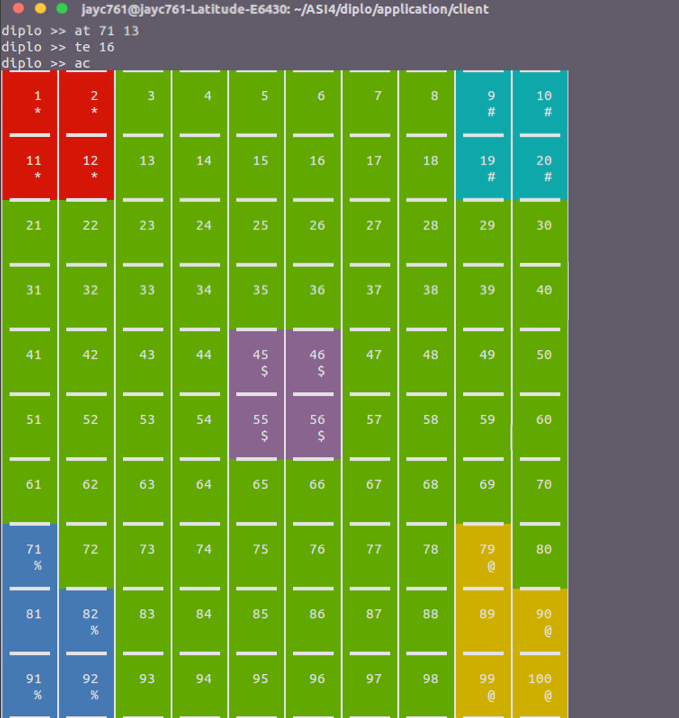
\includegraphics[scale=0.2]{images/carte.png}
					\caption{Carte du client}
				\end{figure}
			\end{column}
		\end{columns}
	\end{frame}
	\begin{frame}[fragile]
		\frametitle{User-Agent}
		\begin{verbatim}
			Diplo/1.0

			Mozilla/5.0 (X11; Linux x86_64) 
			AppleWebKit/537.36 (KHTML, like Gecko) 
			Ubuntu Chromium/41.0.2272.76 
			Chrome/41.0.2272.76 
			Safari/537.36
		\end{verbatim}
	\end{frame}
